\documentclass[handout]{beamer}

\usepackage[frenchb]{babel}
\usepackage[T1]{fontenc}
\usepackage[utf8x]{inputenc}
\usepackage{minted}
 
\usetheme{Berkeley}
\usecolortheme{crane}
\useinnertheme{rounded}

\title{Présentation projet P2 : PHP}
\author{Conrad \bsc{Hillairet} et Alexandre \bsc{Vieira}}
\institute{INSA de Rouen}
\date{14 mai 2012}


\AtBeginSection[]
{
	\begin{frame}
		\frametitle{Sommaire}
		\tableofcontents[currentsection, hideothersubsections]
	\end{frame}
}

\begin{document}

\begin{frame}
\titlepage
\end{frame}

\begin{frame}
	\frametitle{Sommaire}
	\tableofcontents
\end{frame}

\section{Présentation générale}
\subsection[Fonction. global]{Fonctionnement global}
 
\begin{frame}
	\frametitle{HTML vs PHP}
	Différence site classique et dynamique\\
	\begin{center}
		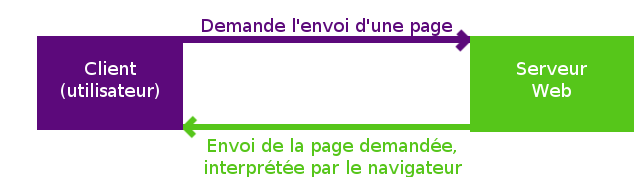
\includegraphics[scale=0.4]{../dossier-HTML.png}

		\bigskip
	\end{center}
\end{frame}

\begin{frame}
	\frametitle{HTML vs PHP}
	Différence site classique et dynamique\\
	\begin{center}
		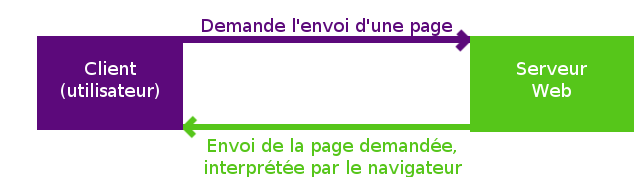
\includegraphics[scale=0.4]{../dossier-HTML.png}

		\bigskip
		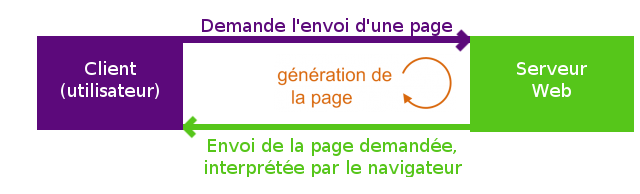
\includegraphics[scale=0.4]{../dossier-PHP.png}
	\end{center}
\end{frame}
 
\subsection{Variables, boucles et conditionnelles}
\begin{frame}
	\frametitle{Les variables}
	\begin{block}{Les variables en PHP}
		\begin{itemize}
			\item Commence par le signe \texttt{\$}
			\item Affectation par le signe \texttt{=}
			\item Pas de déclaration, pas de type
		\end{itemize}
	\end{block}

	\begin{exampleblock}{Exemple}
		\texttt{\$nb = 3}\\
		\texttt{\$cdc = "Hello World !"}
	\end{exampleblock}
\end{frame}
 
\begin{frame}[fragile]
	\frametitle{Les conditionnelles}
	\framesubtitle{if...else...}
	\begin{block}{if...else...}
	Sert essentiellement aux schémas conditionnels simples.
\end{block}

	\begin{alertblock}{Syntaxe}
		\begin{minted}[fontsize=\scriptsize]{php}
			<?php
			if (condition1)
				{
					/*Suite d'instructions si condition1 est vraie*/
				}
				elseif (condition2)
				{
					/*Suite d'instructions si condtion1 est fausse et condition2 est vraie*/
				}
				else
				{
					/*Suite d'instructions si condition1 et condition2 sont fausses*/
				}
			?>
		\end{minted}
	\end{alertblock}
\end{frame}


\begin{frame}[fragile]
	\frametitle{Les conditionnelles}
	\framesubtitle{switch}
	\begin{block}{switch}
	Sert aux schémas conditionnels plus complexes.
	\end{block}

	\begin{alertblock}{Syntaxe}
		\begin{minted}[fontsize=\scriptsize]{php}
			<?php
			switch(variable)
			{
				case valeur1 : //Si variable vaut une certaine valeur
					Instructions;
				case valeur2 :
					Instructions;
				...
				default //Si aucune des conditions ne sont remplies au-dessus
					Instructions;
			}
			?>
		\end{minted}
	\end{alertblock}
\end{frame}

\begin{frame}[fragile]
	\frametitle{Les boucles}
	\framesubtitle{while}
	\begin{block}{while}
		Faire une boucle indeterministe
	\end{block}

	\begin{alertblock}{Syntaxe}
	\begin{minted}[fontsize=\scriptsize]{php}
		<?php
		while (condition)
		{
				//Instructions a realiser tant que condition est vrai
		}
		?>
	\end{minted}
	\end{alertblock}
\end{frame}

\begin{frame}[fragile]
	\frametitle{Les boucles}
	\framesubtitle{while}
	\begin{block}{while}
		Faire une boucle indeterministe
	\end{block}

	\begin{exampleblock}{Exemple}
	\begin{minted}[fontsize=\scriptsize]{php}
		<?php
		$i=0;
		while ($i<10)
		{
			if($i<5)
				echo "<p>", $i, "</p>";
			else
				echo "<h1>", $i, "</h1>";
			$i++;
		}
		?>
	\end{minted}
	\end{exampleblock}
\end{frame}

\begin{frame}[fragile]
	\frametitle{Les boucles}
	\framesubtitle{for}
	\begin{block}{for}
		Faire une boucle déterministe
	\end{block}

	\begin{alertblock}{Syntaxe}
	\begin{minted}[fontsize=\scriptsize]{php}
		<?php
		for ($i=0,;$i<$n;$i++)
		{
				//Instructions a realiser
		}
		?>
	\end{minted}
	\end{alertblock}
\end{frame}

\begin{frame}[fragile]
	\frametitle{Les boucles}
	\framesubtitle{for}
	\begin{block}{for}
		Faire une boucle déterministe
	\end{block}

	\begin{exampleblock}{Exemple}
	\begin{minted}[fontsize=\scriptsize]{php}
		<?php
		for ($i=0;$i<10;$i++)
		{
			if($i<5)
				echo "<p>", $i, "</p>";
			else
				echo "<h1>", $i, "</h1>";
		}
		?>
	\end{minted}
	\end{exampleblock}
\end{frame}


\begin{frame}
	\frametitle{Les fonctions prédéfnies}
	\begin{block}{Les fonctions prédéfinies}
		Nombreuses et de toutes sortes :
		\begin{itemize}
			\item \texttt{echo}
			\item Opérations automatiques sur les variables (\texttt{strlen} ou \texttt{strtolower})
			\item Fonctions mathématiques (\texttt{cos} ou \texttt{rand})
		\end{itemize}
	\end{block}

\end{frame}

\subsection{Les bases de données}
\begin{frame}
	\frametitle{SGBD}

	\begin{block}{SGBD ?}
		\begin{itemize}
			\item L'utilité des bases de données
			\item Les différents Systèmes de Gestion des Bases de Données (SGBD)
			\item Les différences et les points communs
			\item L'utilité du PHP
		\end{itemize}
	\end{block}
\end{frame}

\begin{frame}
	\begin{center}
	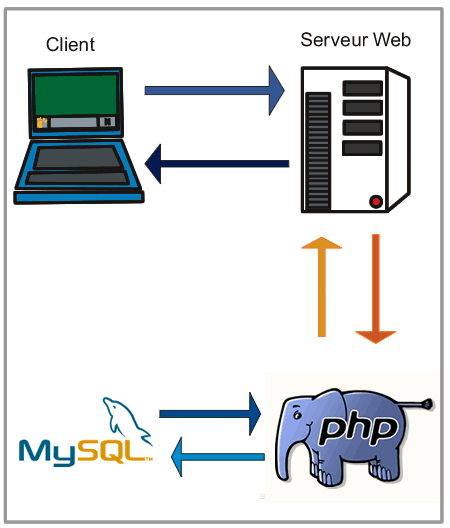
\includegraphics[scale=0.4]{../schema2.png}
	\end{center}
\end{frame}

\begin{frame}
	\frametitle{Organisation des BDD}
	\begin{block}{Nomenclature}
		\begin{itemize}
			\item La base
			\item Les tables
			\item Les champs et les entrées
		\end{itemize}
	\end{block}
\end{frame}

\begin{frame}[fragile]
	\frametitle{Différentes instructions SQL}
	\begin{block}{Connexion à la base de données}
	\begin{minted}[startinline,fontsize=\scriptsize]{php}
	$bdd = new PDO('mysql:host=NomDeLHost;
	dbname=NomDeLaBase', 'NomDUtilisateur', 
	'MotDePasse');
	\end{minted}
	\end{block}

	\begin{exampleblock}{Exemple sur le site}
		\begin{minted}[startinline,fontsize=\scriptsize]{php}
			$bdd = new PDO('mysql:host=mysql2.alwaysdata.com;
			dbname=essaissitesweb_news', '67162', 'penrchalper');
		\end{minted}
	\end{exampleblock}
\end{frame}

\begin{frame}[fragile]
	\frametitle{Différentes instructions SQL}
	\begin{block}{Récupérer les champs}
	\begin{minted}[startinline,fontsize=\scriptsize]{php}
	$reponse = $bdd -> query(SELECT nomDuChamp1 nomDuChamp2 ... 
	FROM NomDeLaTable WHERE CondtionSurUnChamp)
	\end{minted}
	\end{block}

	\begin{exampleblock}{Exemple sur le site}
	\begin{minted}[startinline,fontsize=\scriptsize]{php}
	$req = $bdd->query('SELECT titre, contenu, DATE_FORMAT(date_ecriture,
	\'%d/%m/%Y\') AS date_ecr FROM articles ORDER BY date_ecriture
	DESC LIMIT 0, 10');
	$donnees = $reponse->fetch()
	\end{minted}
	\end{exampleblock}
\end{frame}
 
\begin{frame}[fragile]
	\frametitle{Différentes instructions SQL}

	\begin{block}{Ajouter des données à une table}
	\begin{minted}[startinline,fontsize=\scriptsize]{php}
		$bdd->exec('INSERT INTO NomTable(NomDesChamps) 
		VALUES(ValeurAAffecterAuxChamps)');
	\end{minted}
	\end{block}

	\begin{block}{Ajouter des données variables}
	\begin{minted}[startinline,fontsize=\scriptsize]{php}
		$req = $bdd->prepare('INSERT INTO NomTable(NomDesChamps) 
		VALUES(:identifiants)');
			$req->execute(array('identifiant' => $ValeurVariable,));
	\end{minted}
	\end{block}

	\begin{exampleblock}{Exemple sur le site}
		\begin{minted}[startinline,fontsize=\scriptsize]{php}
		$sauv = $bdd->prepare('INSERT INTO articles(titre, contenu,
		date_ecriture) VALUES(:titre, :contenu, NOW())');
		$sauv->execute(array(
			'titre'=>$_POST['titre'],
			'contenu'=>$_POST['message'],
		));
	\end{minted}
	\end{exampleblock}
\end{frame}


\section{Présentation du site}
\subsection{Objectifs}
 
\begin{frame}
	\frametitle{Principaux objectifs}
	\begin{block}{Contenu du site :}
	\begin{itemize}
		\item Réaliser une page présentant un ensemble de news enregistrées dans une base de données
		\item Créer un formulaire d'ajout de news
		\item Créer un formulaire de contact
	\end{itemize}
	\end{block}
\end{frame}

\subsection{Visite du site}
 
\begin{frame}
	\frametitle{Visite commentée du site}
	\begin{center}
	\href{http://essaissitesweb.alwaysdata.net/}{\beamergotobutton{Lien vers le site}}
	\end{center}
\end{frame}

\section*{Conclusion}
\begin{frame}
	\frametitle{Conclusion}
	\begin{center}
	Avez-vous des questions ?\\
	
\includegraphics[scale=0.5]{elePHPant.jpg}
\end{center}
\end{frame}
\end{document}
